\documentclass[11pt]{article}
\usepackage{graphicx}
\usepackage[english]{babel}
\usepackage{float}
\usepackage{amsmath}
\usepackage[section]{placeins}
\usepackage{hyperref}
\graphicspath{ {./images/} }

\usepackage[T1]{fontenc}
\usepackage{listings}
\usepackage{hyperref}
\usepackage{color}

\definecolor{dkgreen}{rgb}{0,0.6,0}
\definecolor{gray}{rgb}{0.5,0.5,0.5}
\definecolor{mauve}{rgb}{0.58,0,0.82}

\lstset{frame=tb,
  language=C++,
  aboveskip=3mm,
  belowskip=3mm,
  showstringspaces=false,
  columns=flexible,
  basicstyle={\small\ttfamily},
  numbers=none,
  numberstyle=\tiny\color{gray},
  keywordstyle=\color{blue},
  commentstyle=\color{dkgreen},
  stringstyle=\color{mauve},
  breaklines=true,
  breakatwhitespace=true,
  tabsize=3
}

\setlength{\parindent}{0pt}
\setlength{\parskip}{0pt plus 0.5ex}
%% adjust spacing for all itemize/enumerate

\begin{document}


\tableofcontents

% TODO: add in more links whenever possible
\section{Useful Resources}
Robot modelling in urdf is rather tedious. Here are a couple of guides/tips which I have found useful.


\begin{itemize}
 \item {
       \href{https://nu-msr.github.io/me495_site/lecture06_modeling.html}{URDF/xacro guide}
       }
 \item{
       \href{   https://classic.gazebosim.org/tutorials?tut=ros_gzplugins}{Guide for gazebo plugins (used to simulate sensors/actuators in gazebo)}
       }
 \item{
       \href{
        https://medium.com/teamarimac/integrating-sonar-and-ir-sensor-plugin-to-robot-model-in-gazebo-with-ros-656fd9452607
       }{Sonar Plugin Guide}
       }
 \item{
       This is a folder which contains many gazebo .world files.
       \begin{lstlisting}[language=bash]
        /usr/share/gazebo-9/worlds
       \end{lstlisting}
       }
       
\end{itemize}
\section{Useful Tools}
\begin{itemize}
 \item {Fusion 360 - A CAD software. Quite useful for measuring the dimensions of mesh files }
 \item { Mesh Lab - A piece of software to visualise and manipulate mesh files.}
\end{itemize}


\section{Installation}
\begin{enumerate}
 \item{Install the joint state publisher:
       \begin{lstlisting}[language=bash]
$ sudo apt install ros-melodic-joint-state-publisher-gui
       \end{lstlisting}
       }
 \item {
       Next, git clone the \textbf{lb\_msgs} package into your catkin/src folder.
       }
 \item{
       Next, git clone realsense package into your catkin/src folder.
       \begin{lstlisting}[language=bash]
$ git clone https://github.com/SynapseProgramming/realsense_gazebo_plugin.git
       \end{lstlisting}
       }
       
 \item{
       % https://github.com/SynapseProgramming/map2gazebo.git
       Next, git clone the map2gazebo package into your catkin/src folder
       
       \begin{lstlisting}[language=bash]
$ git clone https://github.com/SynapseProgramming/map2gazebo.git
       \end{lstlisting}
       }
       
       
 \item{
       Enter the following command into the terminal to setup gazebo environment variables
       \begin{lstlisting}[language=bash]
       $ echo "source /usr/share/gazebo/setup.sh" >> ~/.bashrc
       $ source ~/.bashrc
       \end{lstlisting}
       
       }
 \item{
       Lastly, remember to run the cakin\_make command.
       }
       
       % TODO: add in the fake_world package once done.
       % add back the excluded stl mesh files.
       % not sure if this package should be stored in gitlab or gitub
\end{enumerate}

\section{Package Overview}
\subsection{world}
The world folder is used to store gazebo .world files. .world files are used to describe the surrounding environment in Gazebo.
\subsection{urdf}
The urdf folder is used to store (.urdf.xacro) and (.gazebo.xacro) files.
\begin{itemize}
 \item {
       (.urdf.xacro) files describe the transformations between the various links of the robot, along with other variables such as intertia.
       }
 \item{
       (.gazebo.xacro) files would describe the kinematic properties of the robot such as velocity limits, coefficient of friction etc.
       }
\end{itemize}
\subsubsection{Intel Realsense D435 camera}
\begin{itemize}
 \item {
       The (\_d435.gazebo.xacro) file is used to describe the various kinematic properties of the depth camera.
       }
 \item{
       The (\_d435.urdf.xacro) file is used to describe the various frames of the depth camera.
       
       The (<camera>\_bottom\_screw\_frame) is used as the main reference point for the depth camera. It is centered about the bottom tripod mount of the depth camera.
       Thus, to define the position of the depth camera on the robot, we would have to provide the transformation from base link to the bottom screw frame link
       }
\end{itemize}
\subsubsection{cub\_full\_robosense.urdf.xacro}
Cub with a robosense Helios-5515 3D lidar.
\subsubsection{cub\_full\_urdf.xacro}
Cub complete with all depth cameras, sonar, bumper and lidar sensors.
\subsubsection{cub\_full\_shifted\_urdf.xacro}
URDF file used to test camera extrinsics calibration.
\subsubsection{cub\_full\_issac\_urdf.xacro}
URDF file used to test issac sim stuff.

\subsection{meshes}
The meshes folder is used to store the various mesh files of the robot(.stl .dae).
The mesh files are used to visualize various components of the robot(sensors, chassis) and to enable accurate collisions within gazebo.

\subsection{rviz}
The rviz folder is used to store the various rviz configs.

% TODO: update launch section when more launch files are created
\subsection{launch}
\begin{itemize}
 \item{
       
       The launch folder is used to store roslaunch files. Launch files titled simulate\_<robotname>.launch are used to launch the gazebo simulation environment and rviz.
       }
 \item{
       Launch files titled view\_<robot>.launch are used to view the robots urdf model in rviz.
       }
 \item{
       Launch files titled <stuff>\_robosense.launch are used to launch cub models with a robosense Helios 3D lidar.
       }
\end{itemize}


% TODO: complete the section on how to scale and manipulate stl files so that the mesh could be easily integrated into rviz

\section{Mesh Manipulation}
\subsection{Reducing the quality of a mesh (Mesh Lab)}
In most cases, the generated meshes are too large for gazebo to render at a high framerate. Thus, we would have to reduce the resolution of our meshes.
\begin{enumerate}
 \item {
       Open meshlab and import the mesh (file > import mesh)
       }
 \item{
       Click on Filters > Remeshing, Simplification and Reconstruction >  Quadratic edge collapse decimation
       }
 \item{
       Select a lower number of (target number of faces) and click apply.
       }
 \item{
       click on file > export mesh as > (enter mesh name and select \emph{.stl} file type)
       }
\end{enumerate}
\subsection{Scaling Down a mesh (Fusion 360) }
\begin{enumerate}
 \item {
       Click on insert > insert mesh
       }
 \item {
       Select the correct units for the given mesh and select center position.
       }
 \item {
       Click on mesh > modify > scale mesh
       }
 \item {
       Click on the mesh and apply a scale factor of 0.1
       }
 \item {
       Repeat steps 3 and 4 repeatedly until the desired scale factor is achieved (for example, this process would have to be repeated 3 times to scale from \emph{mm} to \emph{m} )
       }
 \item{
       Save the project, and export the final mesh as a .stl file.
       }
\end{enumerate}

\subsection{Mesh Origin}
Each stl file has a origin. In most cases, we would want to modify the origin for various reasons.

\subsubsection{Centering a mesh}
\begin{enumerate}
 \item {
       Import a mesh into meshlab.
       }
 \item{
       click on render > show axis
       }
 \item{
       click on filters > Normals Curvature and Orientation > Transform: Move, Translate, Center
       }
 \item{
       Select translate center of bbox to the origin and click apply.
       
       }
       
\end{enumerate}
\emph{In most cases, the centered origin is used to as the centre of mass. Thus, intertia is computed with respect to the centered origin.}
\subsubsection{Translating \& rotating a mesh}
\begin{itemize}
 \item {
       Under filters > Normals Curvature and Orientation, there are a few transform operations which could carried out on the mesh.
       }
\end{itemize}

\emph{Do take note of the translation between the center origin of the mesh, and the final origin of the mesh as we would have to take that into account when defining the intertia reference frame.}
\section{Computing Intertia of meshes}
In Gazebo, the inertia parameters should be well defined as they are used by the physics engine.
Incorrect inertia parameters may result in odd occurences such as sliding on the spot.
\subsection{Key Variables}
\begin{itemize}
 \item {
       scaling factor $s$
       \begin{itemize}
        \item {URDF uses $m$ (metres) to measure distance.}
        \item{ Most \emph{.stl} files would be in $mm$ (milimetres) }
        \item{In this example, scaling factor $s=10^2$ (the .stl file is in $cm$)}
       \end{itemize}
       }
 \item{
       Mesh Origin
       
       The center origin of the mesh would be used as the reference frame for intertia.
       
       Therefore, if the center origin of the mesh is not used as the main origin for the current part, we would have to
       specify the translation from the main origin to the center origin.
       
       
       \begin{figure}[!htb]
        \centering
        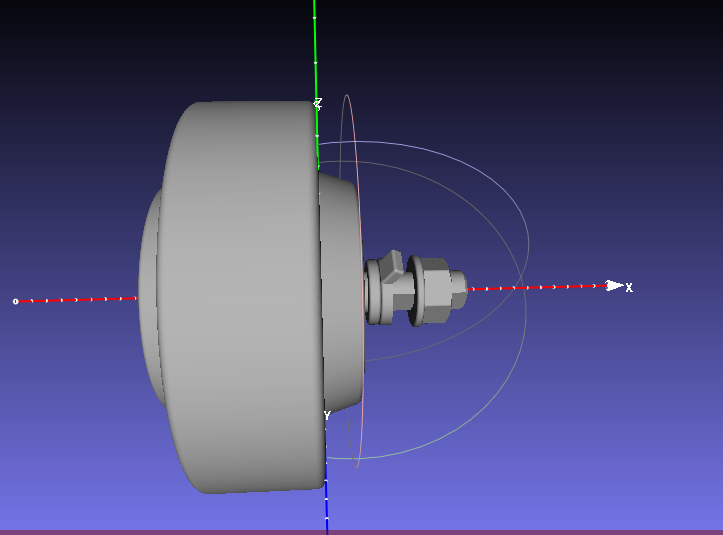
\includegraphics[width=0.5\textwidth]{images/centeredwheel}
        \caption{Wheel mesh with centered origin}
       \end{figure}
       
       
       \begin{figure}[!htb]
        \centering
        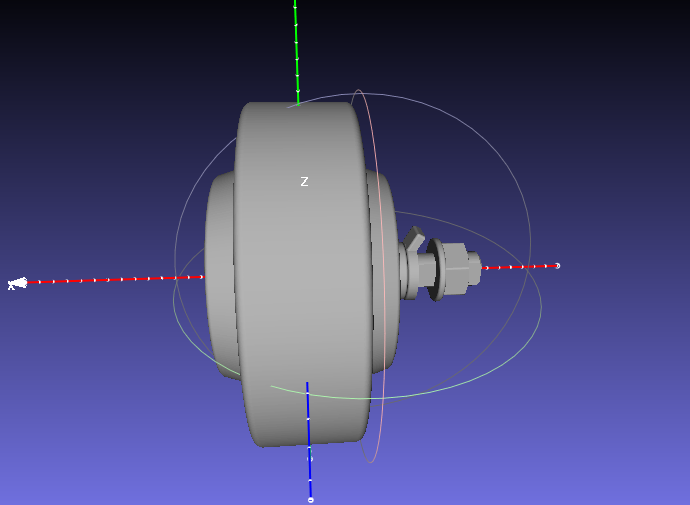
\includegraphics[width=0.5\textwidth]{images/offcenteredwheel}
        \caption{Wheel mesh with off-centered origin}
       \end{figure}
       }
\end{itemize}
\subsection{Computing Intertia }
\begin{enumerate}
 \item {Firstly, import the mesh into meshlab.}
 \item{Ensure that the current origin of the mesh is its center.}
 \item{ Click on filters > Cleaning and Repairing > Remove Duplicate Faces}
 \item{ Click on view > Show Layer Dialog (ensure that a right window pops up)}
 \item {Click on filters > Quality measure and computations > Compute Geometric Measures}
 \item {
       At the bottom right corner, the following text would be generated.
       \begin{lstlisting}[language=bash]

        Mesh Bounding Box Size 10.275001 13.000000 13.000000
        Mesh Bounding Box Diag 21.061235
        Mesh Volume is 575.673584
        Mesh Surface is 1340.176147
        Thin shell barycenter -0.288410 0.036296 0.007559
        Center of Mass is -0.142327 0.002174 0.000383
        Inertia Tensor is :
        | 10287.553711 2.708627 0.324480 |
        | 2.708627 6752.031738 -0.408094 |
        | 0.324480 -0.408094 6754.208984 |
        Principal axes are :
        | 1.000000 -0.000770 0.000046 |
        | 0.000766 0.983973 -0.178316 |
        | 0.000092 0.178316 0.983973 |
        axis momenta are :
        | 10287.555664 6751.955566 6754.282715 |

       \end{lstlisting}
       \begin{itemize}
        \item {
              The Intertia Tensor generated by MeshLab would correspond to the following matrix
              $$
               \begin{bmatrix}
                I_{xx} & I_{xy} & I_{xz} \\
                I_{xy} & I_{yy} & I_{yz} \\
                I_{xz} & I_{yz} & I_{zz} \\
               \end{bmatrix}
              $$
              }
        \item{
              As the mesh used in this example is in $cm$, the mesh volume would be in ${cm}^3$
              }
       \end{itemize}
       
       }
\end{enumerate}
\subsection{Importing Inertia Values into URDF}
\begin{enumerate}
 \item {
       Let $v$ be the volume of the mesh in $m^3$
       
       As the generated mesh volume is in ${cm}^3$, we would have to multiply the mesh volume by $10^{-6}$ to scale it to $m^3$.
       
       $v=575.673584\times10^{-6}$
       }
 \item {
       Let $m$ be the mass of the given object in $kg$
       
       In this case, we will assume that the wheel weighs $5kg$
       }
 \item {
       
       Each element in the inertia matrix would have to be scaled down by $s^5$, where $s$ is the scaling factor.
       (eg. s=$10^2$ for a mesh in $cm$. Thus, each $I$ value would have to be multiplied by $10^{-10}$)
       
       Furthermore, each element in the inertia matrix would have to be multiplied by mass $m$ and divided by volume $v$
       
       $$
        \frac{m}{vs^5}
        \begin{bmatrix}
         I_{xx} & I_{xy} & I_{xz} \\
         I_{xy} & I_{yy} & I_{yz} \\
         I_{xz} & I_{yz} & I_{zz} \\
        \end{bmatrix}
       $$
       }
 \item{
       Next, we would have to fill up the inertia tag in the URDF file.
       \begin{itemize}
        \item { \emph{origin} tag should be filled with the translation from the main origin to the center origin (if neccessary)}
        \item { \emph{inertia} tag should be filled with the scaled inertia values. }
        \item { \emph{mass} tag should be filled with mass $m$.}
       \end{itemize}
       \begin{lstlisting}[language=bash]
    <inertial>
      <origin xyz="0 0 0"/>
      <mass value="5"/>
      <inertia ixx="0.00893523" ixy="2.35258e-06" ixz="2.81826e-07" iyy="0.00586446" iyz="-3.54454e-07" izz="0.00586635"/>
    </inertial>
       \end{lstlisting}
       }
 \item {
       In the simulation, the center of mass may cause the robot to drift forward. Therefore, the origin inertia tag should be tuned if needed.
       }
\end{enumerate}
\subsection{Verifying Inertia Values}
If the inertia values were computed correctly, then the mesh should have a pink box surrounding the mesh in Gazebo (view > inertia)
\begin{figure}[H]
 \centering
 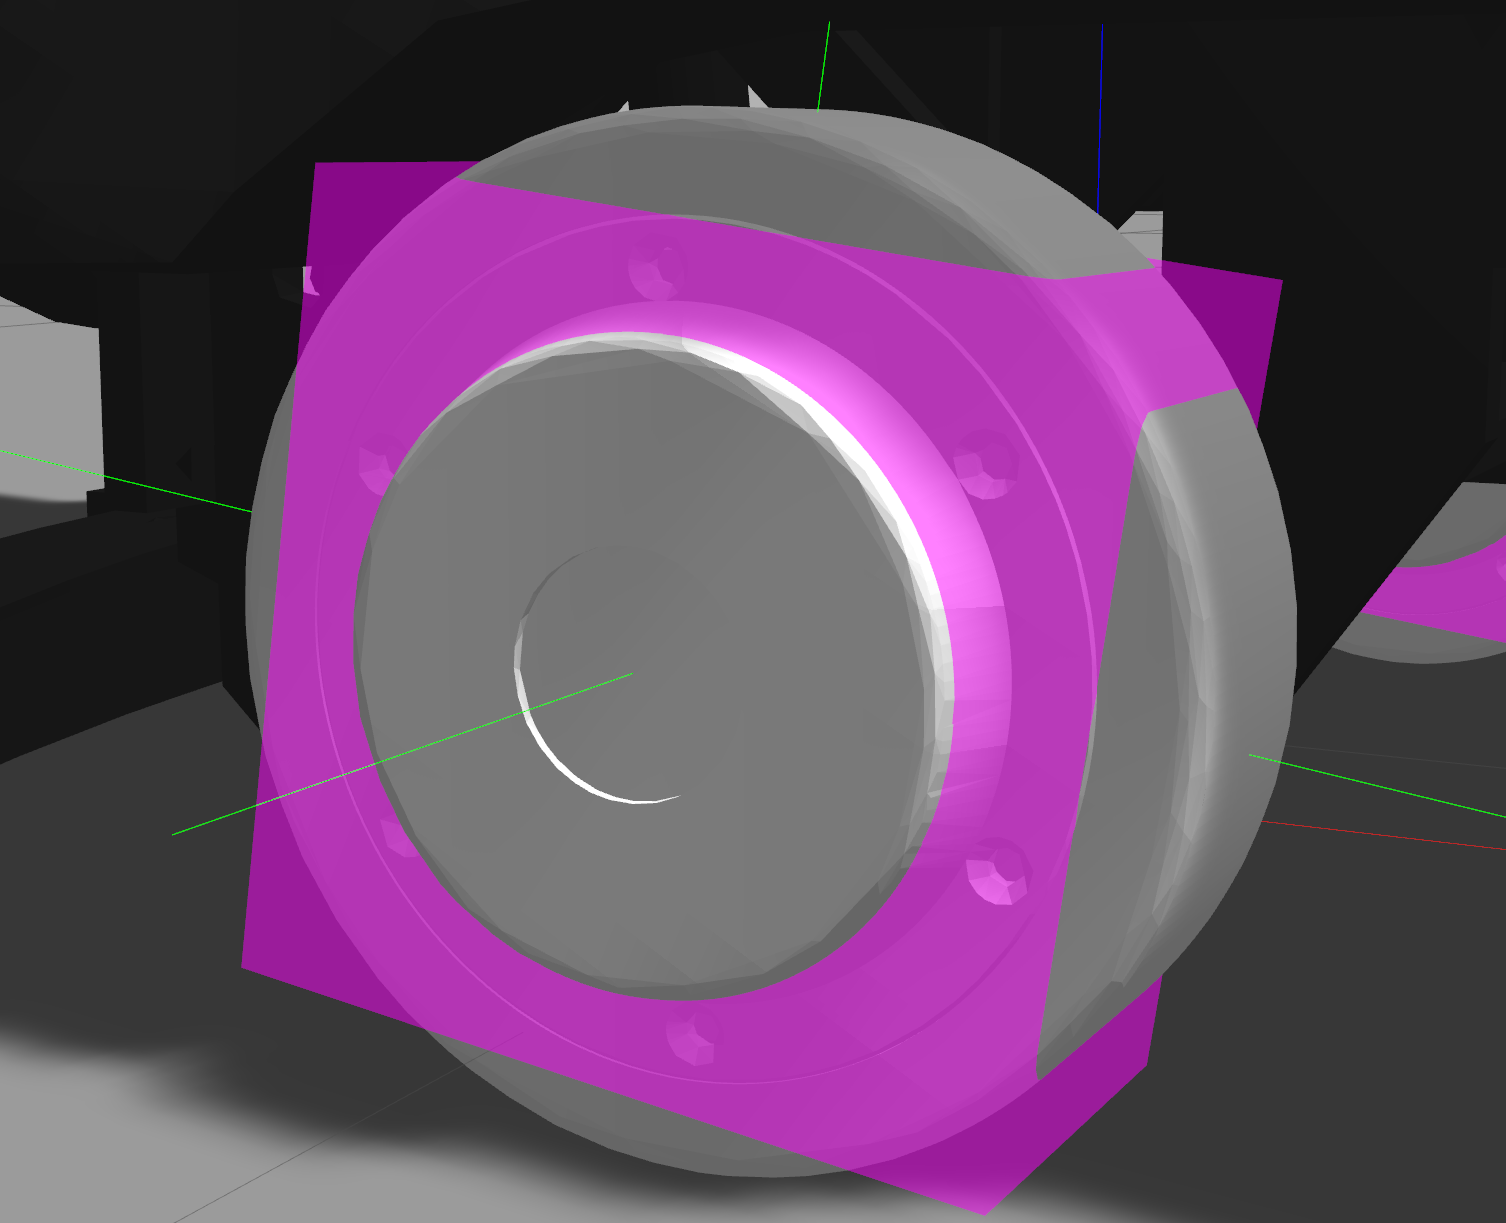
\includegraphics[width=0.5\textwidth]{images/inertiawheel}
 \caption{Wheel with inertia bounding box}
\end{figure}

\subsection{Closed Inertia Formulas}
\subsubsection{Solid Sphere}
\begin{itemize}
 \item {
       $m$ Mass in \emph{kg}
       }
       
 \item {
       $r$ radius of sphere in metres
       }
\end{itemize}

$$
 \begin{bmatrix}
  I_{xx}=\frac{2}{5}mr^2 & I_{xy}=0               & I_{xz}=0               \\
  I_{xy}=0               & I_{yy}=\frac{2}{5}mr^2 & I_{yz}=0               \\
  I_{xz}=0               & I_{yz}=0               & I_{zz}=\frac{2}{5}mr^2 \\
 \end{bmatrix}
$$


\section{Gazebo World from 2D Map}
\subsection{Setup \& Installation}

\begin{enumerate}
 \item{
       Ensure that the map server is installed on your system.
       \begin{lstlisting}[language=bash]
     $ sudo apt install ros-melodic-map-server
       \end{lstlisting}
       }
 \item{
       Clone the \href{https://github.com/SynapseProgramming/map2gazebo.git
       }{\emph{map2gazebo}} repository into your catkin/src folder.
       
       }
 \item{
       Navigate to the \emph{map2gazebo} package in your catkin/src folder and run the following commands.
       
       \begin{lstlisting}[language=bash]
         $ pip install --user trimesh
         $ pip install --user numpy
         $ pip install --user pycollada
         $ pip install --user scipy
         $ pip install --user networkx
       \end{lstlisting}
       }
 \item{
       Lastly, navigate to your catkin\_ws folder and run catkin\_make
       }
\end{enumerate}

\subsection{Generation of map.stl file}

\begin{enumerate}
 \item{launch roscore}
 \item {
       Navigate to the folder containing the \emph{pgm} and \emph{yaml} file for the map that you would want to convert and run the following command to launch the map server.
       \begin{lstlisting}[language=bash]
        $ rosrun map_server map_server <map name>.yaml
       \end{lstlisting}
       }
 \item{
       Then, run the following command to generate the \emph{map.stl} at a given directory. (replace
       \emph{/home/roald/Desktop/generatedmaps} with your own path)
       
       \begin{lstlisting}[language=bash]
        $ roslaunch map2gazebo map2gazebo.launch export_dir:=/home/roald/Desktop/generatedmaps
        \end{lstlisting}
       }
\end{enumerate}
\subsection{Importing the mesh into Gazebo}
\begin{enumerate}
 \item {
       Firstly, navigate to the following directory
       \begin{lstlisting}[language=bash]
 catkin_ws/src/map2gazebo/models/map/meshes
        \end{lstlisting}
       }
 \item {
       Replace the existing map.stl file with the newly generated map.stl file.
       }
 \item{
       Launch the following command to launch the gazebo simulation with the current robot in the new map.
       \begin{lstlisting}[language=bash]
       $ roslaunch fake_world simulate_cub_lab.launch
        \end{lstlisting}
       
       }
\end{enumerate}

\section{multimaster\_fkie}
Multimaster\_fkie is a collection of packages which allows topics to be passed between separate devices, while running separate masters.


\subsection{Networking}
\begin{itemize}
 \item { All machines should be connected to the same local network}
 \item{ DHCP reservation could be used to ensure that the machines have a static IP address}
\end{itemize}
\subsection{Package Installation }
\begin{enumerate}
 \item {
       Enter the following lines to install the package dependencies.
       \begin{lstlisting}[language=bash]
       $ sudo add-apt-repository ppa:roehling/grpc
       $ sudo apt update
       $ pip install grpcio
       $ pip install grpcio-tools
        \end{lstlisting}
       }
 \item{
       Next, navigate to your catkin/src folder and run the following command.
       \begin{lstlisting}[language=bash]
         $ git clone https://github.com/fkie/multimaster_fkie.git
        \end{lstlisting}
       }
 \item{
       Lastly, run catkin\_make to build the package.
       }
       % roslaunch fkie_master_discovery master_discovery.launch
\end{enumerate}
\subsection{Setup \& Usage}

In this section, we shall assume that we would want to pass data between two machines, \emph{M1} and \emph{M2}.

\begin{enumerate}
 \item {
       Ensure that the multimaster\_fkie package is installed on both machines.
       }
 \item {
       Ensure that only one networking option is enabled (either wifi or ethernet)
       }
 \item{
       Next, run the \emph{ifconfig} command on \emph{M1} and \emph{M2} and note down the  assigned ip address.
       }
 \item{
       Next, navigate to the \emph{etc} directory and run the following command
       \begin{lstlisting}[language=bash]
        $ sudo gedit hosts
        \end{lstlisting}
       }
 \item{
       Add the ip addresses of M1 and M2 to the hosts file (replace the fake ip-addresses with real ones and replace \emph{M1} and \emph{M2} with the names of your machines)
       
       (example hosts file for \emph{M1})
       \begin{lstlisting}[language=bash]
       127.0.0.1 localhost
       127.0.1.1 M1

       #for ROS multimaster
       12.13.14.15 M1
       14.13.153.134 M2
        \end{lstlisting}
       }
 \item{
       Repeat steps 3 and 4 on  the other machine. (eg. \emph{M2})
       }
 \item{
       Ensure that roscore is running on both machines \emph{M1} and \emph{M2}
       }
 \item{
       Run the following commands in separate terminals to sync up the two rosmasters on \emph{M1} and \emph{M2}
       \begin{lstlisting}[language=bash]
         $ rosrun fkie_master_discovery master_discovery
         $ roslaunch fkie_master_sync master_sync.launch
        \end{lstlisting}
       
       }
\end{enumerate}
\subsection{Testing}
\begin{enumerate}
 \item {
       Firstly, ensure that roscore, the discovery and the master sync nodes are running on both machines \emph{M1} and \emph{M2}.
       }
 \item{
       Next, run the following command to check if both masters are known by the discovery node.
       Ideally, both masters on the separate machines should be listed here.
       \begin{lstlisting}[language=bash]
         $ rosservice call /master_discovery/list_masters
        \end{lstlisting}
       }
 \item{
       Next, run the following command in \emph{M1} to run the turtlesim node.
       \begin{lstlisting}[language=bash]
          $ rosrun turtlesim turtlesim_node
        \end{lstlisting}
       }
 \item{
       Next, run the following command in \emph{M2} to run the turtlesim teleop node.
       \begin{lstlisting}[language=bash]
          $ rosrun turtlesim turtle_teleop_key
        \end{lstlisting}
       }
 \item{
       Thus, if all went well, pressing the arrow keys on \emph{M2} should move the turtle on \emph{M1}.
       }
\end{enumerate}
\section{Gzweb}
\subsection{Setup \& Installation}
\begin{enumerate}
 \item {
       Firstly, open a new terminal and enter the following commands.
       you may wish to refer to \href{https://classic.gazebosim.org/tutorials?tut=gzweb_install&cat=gzweb}{\emph{this gazebo webpage}}
       \begin{lstlisting}[language=bash]
$ sudo apt install gazebo9 libgazebo9-dev
$ sudo apt install libjansson-dev libboost-dev imagemagick libtinyxml-dev mercurial cmake build-essential
$ curl -o- https://raw.githubusercontent.com/nvm-sh/nvm/v0.35.3/install.sh | bash
$ source ~/.bashrc
$ nvm install 8
$ cd ~; git clone https://github.com/osrf/gzweb
$ cd ~/gzweb
$ git checkout gzweb_1.4.1
$ npm run deploy --- -m
       \end{lstlisting}
       }
 \item{
       Next, navigate to the gzweb/http/client/assets directory.
       \begin{enumerate}
        \item {
              Copy the media directory into the assets directory.
              \begin{lstlisting}[language=bash]
$ cp -R /usr/share/gazebo-11/media gzweb/http/client/assets/
              \end{lstlisting}
              }
        \item{
              Copy all of the meshes within lb\_simulation/meshes to the assets folder.
              }
        \item {
              Copy the entire lb\_description package to the assets folder.
              }
       \end{enumerate}
       }
 \item { Navigate to the gzweb directory and run \emph{npm run deploy --- -m local}}
 \item { Navigate to the gzweb directory and run \emph{npm install}}
\end{enumerate}
\subsection{Usage}
\begin{enumerate}

 \item { Navigate to the gzweb directory and run \emph{npm start}}
 \item{
       Lastly, ensure that the launch file in the simulation package has the GUI tag disabled, before proceeding to enter the roslaunch command.
       \begin{lstlisting}[language=bash]
          <arg name="gui" value="false"/>
       \end{lstlisting}
       }
 \item{
       In order to view the gzweb page on another machine, the URL should be <ip address of server>:8080
       }
\end{enumerate}

\section{Animating Models in Gazebo}
\begin{itemize}
 \item {
       To animate models in Gazebo, we would have to write a model plugin, and specify that plugin from within the model tag.
       }
 \item {
       In the world file, the name of the plugin would be
       lib<name of plugin in Cmake>.so
       
       \begin{lstlisting}[language=bash]
         #in CMake
         add_library(movebox src/movebox.cc)
         #In .world file
        <plugin name="push_animate" filename="libmovebox.so"/>
       \end{lstlisting}
       
       }
\end{itemize}
\section{Converting from urdf.xacro to urdf \& sdf}
\label{sec:conversion}
\begin{enumerate}
 \item {
       To convert a existing urdf.xacro file to a urdf file, please run the following command (and replace
       bot with the name of your file)
       \begin{lstlisting}[language=bash]
$ xacro bot.urdf.xacro > bot.urdf
\end{lstlisting}
       }
 \item {
       To convert a existing urdf file to a sdf file, please run the following command (and replace
       bot with the name of your file)
       \begin{lstlisting}[language=bash]
$ gz sdf -p bot.urdf > bot.sdf
\end{lstlisting}
       }
       
\end{enumerate}

\section{RoboSense Helios-5515 3D lidar}

\subsection{Installation}
\begin{enumerate}
 \item {Firstly, git clone the \textbf{robosense\_simulator\_Helios\_5515} package into your catkin/src folder and run catkin\_make}
 \item{
       \textbf{(optional) update gazebo to version 9.4.0++}
       
       \begin{itemize}
        \item { This step is required if you want the GPU to compute the pointcloud.}
        \item {
              \textbf{If you do not carry out this step, please set \emph{gpu="false"} in the \emph{xacro::RS-5515 tag}
              }
              
              }
        \item{
              Navigate to the robosense\_simulator\_Helios\_5515 directory and refer to \emph{gazebo\_upgrade.md} for a more detailed explanation on the upgrade process.
              }
       \end{itemize}
       }
\end{enumerate}
\subsection{Usage}
\begin{itemize}
 \item {
       After installing the package, please add the following lines to your robots \emph{.urdf.xacro} file.
       \begin{lstlisting}[language=xml]

  <xacro:include filename="$(find robosense_description)/urdf/RS-5515.urdf.xacro"/>

  <xacro:RS-5515 parent="base_link" name="helios" hz="10" samples="1800" gpu="true" noise="0.002">
    <origin xyz="0 0 1.35" rpy="0 0 0"/>
  </xacro:RS-5515>
\end{lstlisting}
       }
 \item{
       You may wish to refer to the \emph{example.urdf.xacro} file which can be found in the \emph{urdf} directory of the Robosense simulator package.
       
       }
\end{itemize}
\section{How to add collision checks (bumper sensors) in Gazebo}
\begin{enumerate}
 \item {
       The first step would be to add the following sensor tag to a gazebo reference (link).
       
       Do change the tags accordingly.
       \begin{lstlisting}[language=xml]
  <gazebo reference="left_bumper">
    <sensor type="contact" name="left_bumper_contact_sensor">
      <selfCollide>true</selfCollide>
      <update_rate>10.0</update_rate>
      <always_on>1</always_on>
      <contact>
        <collision>
          base_footprint_fixed_joint_lump__left_bumper_collision_8
        </collision>
      </contact>
      <plugin name="gazebo_ros_bumper_controller" filename="libgazebo_ros_bumper.so">
        <bumperTopicName>/left_bumper</bumperTopicName>
        <update_rate>10.0</update_rate>
        <always_on>1</always_on>
        <frameName>base_link</frameName>
      </plugin>
    </sensor>
  </gazebo>
\end{lstlisting}
       }
 \item {
       The collision tag is slightly problematic. To fill up the collision tag properly, please generate the
       sdf file of your robot model by following the steps in \hyperref[sec:conversion]{\textbf{this}} section.
       }
 \item {
       Next, open up the generated \emph{.sdf} file and ctrl+f the name of your link. Copy the name of your link which ends with \emph{\_collision\_X} and paste it in the collisions tag.
       
       }
\end{enumerate}
\section{RMF Traffic Editor}
RMF traffic editor is a tool for generating worlds in gazebo.
\subsection{Installation}
RMF traffic editor is a ROS2 based package. As such, do ensure that you have sourced the correct ROS2 setup.bash files.
\subsubsection{System Requirements}
\begin{itemize}
 \item {ROS2 Foxy}
 \item {Ububtu 20.04}
\end{itemize}
\subsubsection{Package Installation}
\begin{enumerate}
 \item{
       Install python3 dependencies
       \begin{lstlisting}[language=bash]
         $ pip install shapely fiona rtree pyproj
        \end{lstlisting}
       }
 \item {
       Clone and install the rmf utils package to your \textbf{colcon workspace}
       \begin{lstlisting}[language=bash]
        $ git clone https://github.com/open-rmf/rmf_utils.git
        \end{lstlisting}
       }
 \item {
       Clone and install the rmf traffic editor package to your \textbf{colcon workspace} and run colcon build.
       \begin{lstlisting}[language=bash]
         $ git clone https://github.com/open-rmf/rmf_traffic_editor.git
        \end{lstlisting}
       
       }
 \item {
       Open up a new terminal and run the following command to launch traffic editor.
       \begin{lstlisting}[language=bash]
         $ traffic-editor
        \end{lstlisting}
       }
 \item {
       Once traffic editor has been launched, click on edit -> preferences
       and select the following file path for thumbnails.
       \begin{lstlisting}[language=bash]
       <workspace_dir>/install/traffic_editor_assets/share/assets/thumbnails
        \end{lstlisting}
       }
\end{enumerate}
\subsection{Map Generation}
Please refer to
\href{ https://osrf.github.io/ros2multirobotbook/traffic-editor.html}{\textbf{this}} document about the basic functions of traffic editor.
\subsubsection{1 Floor Map Generation}
\begin{enumerate}
 \item {Click on the \textbf{levels} tab and click add}
 \item {Provide a suitable map image and map name.}
 \item {Add walls}
 \item {Add a floor polygon (\textbf{save and re-launch} traffic editor to view the floor polygon)}
 \item {
       Add a single \textbf{measurement} in the map (pink line between vertices)
       
       Measurement is the distance between two vertices in the map (eg. a wall represented by two vertices on each end and one edge that connects them). A incorrect measurement would result in map scaling issues.
       
       \begin{figure}[H]
        \centering
        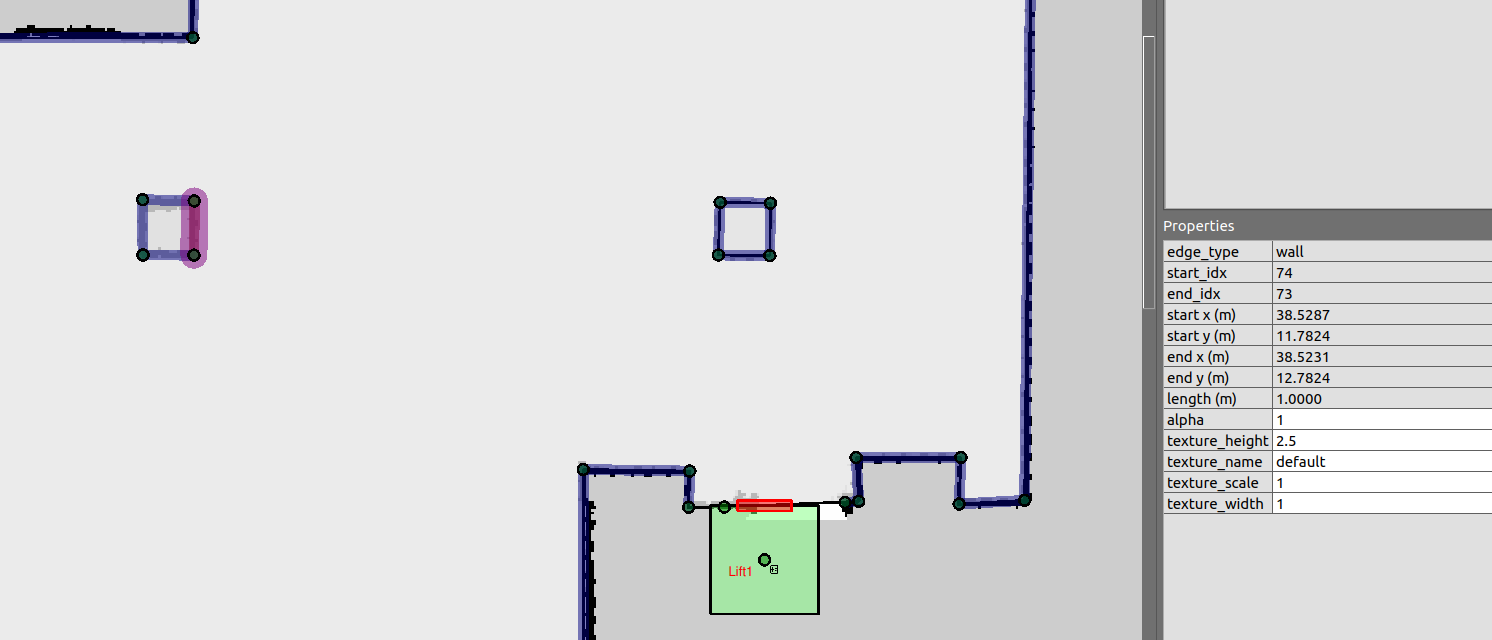
\includegraphics[width=0.9\textwidth]{images/dimension}
        \caption{Dimension (in pink) of column (width of 1 metre in real life)}
       \end{figure}
       }
 \item {Save the map. (ensure that the building.yaml file is generated)}
\end{enumerate}
\subsubsection{Export to simulation package}
\begin{enumerate}
 \item {Navigate to the directory which contains the <worldname>.building.yaml file.}
 \item {
       Run the following command to generate the <worldname>.world file and <worldname> mesh folder.
       \begin{lstlisting}[language=bash]
        $ ros2 run rmf_building_map_tools building_map_generator gazebo <worldname>.building.yaml <worldname>.world .
        \end{lstlisting}
       }
 \item {
       \begin{itemize}
        \item {
              Copy the generated <worldname>.world file into the world folder of the simulation package.
              }
        \item {
              Copy the generated <worldname> mesh folder into the meshes folder of the simulation package.
              }
       \end{itemize}
       }
\end{enumerate}
\subsubsection{Modify Wall Height}
\begin{enumerate}
 \item {open the wall.py file (available at):
       \begin{lstlisting}[language=bash]
         rmf_traffic_editor > rmf_building_map_tools > building_map > wall.py
        \end{lstlisting}
       }
 \item {
       Modify the wall height at line 16
       \begin{lstlisting}[language=python]
        self.wall_height = 2.5  # meters
        \end{lstlisting}
       }
 \item {Run colcon build}
 \item{
       Rebuild the <worldname>.world and mesh files
       }
\end{enumerate}
\subsection{Add custom meshes}
To add custom meshes into RMF traffic editor, we would have to generate their thumbnails. Thumbnails are top down views of a mesh model.

Gazebo-compatible meshes could be downloaded from \href{https://app.gazebosim.org/dashboard}{\emph{this}} website.
\subsubsection{Thumbnail Generation}
\begin{enumerate}
 \item {
       Navigate to the folder of the model to be imported into traffic editor. (It should contain a model.sdf file)
       }
 \item {
       Run the following command.
       \begin{lstlisting}[language=bash]
         $ gzserver -s libthumbnail_generator.so empty.world --verbose --input <model filepath>/model.sdf --output .
        \end{lstlisting}
       A single .png image should be generated. (It would have the same name as the generated mesh)
       }
 \item {
       Next, navigate to the following directory (within the traffic editor ROS2 package), and create a new directory called Custom.
       \begin{lstlisting}[language=bash]
rmf_traffic_editor/rmf_traffic_editor_assets/assets/thumbnails/images/cropped
        \end{lstlisting}
       }
       Paste all generated thumbnails in the Custom folder.
 \item  {
       Next, navigate to the following directory (within the traffic editor ROS2 package)
       \begin{lstlisting}[language=bash]
rmf_traffic_editor/rmf_traffic_editor_assets/assets/thumbnails
        \end{lstlisting}
       }
 \item {
       Insert the new thumbnails into the model\_list.yaml file. (eg. shelf is a new thumbnail.)
       \begin{lstlisting}[language=bash]
  meters_per_pixel: 0.004
models:
- Custom/Shelf
- Custom/aws_robomaker_warehouse_ShelfF_01
- Custom/aws_robomaker_warehouse_ShelfE_01
- OpenRobotics/AdjTable
- OpenRobotics/AirportBench
...
  \end{lstlisting}
       }
 \item {
       Lastly, run colcon build. The meshes should be available in traffic editor.
       }
\end{enumerate}
\subsubsection{Custom meshes in Gazebo}
In order for meshes to be loaded in gazebo, they have to be placed in the meshes directory
of the lb\_simulation package.
\begin{lstlisting}[language=bash]
<workspace>/src/lb_simulation/lb_simulation/meshes
\end{lstlisting}

\end{document}
